% <<FF>> ***********************************************************************
% https://www.overleaf.com/learn/latex/Beamer_Presentations:_A_Tutorial_for_Beginners_(Part_2)%E2%80%94Lists,_Columns,_Pictures,_Descriptions_and_Tables#The_Description_Environment
\begin{frame}
  \frametitle{TikZ Test}

  Hello world


% <<FF>> ********************************************************************
% FIGURE: Linear Approximation of the measured curves
% ***************************************************************************
% \begin{figure}[htbp]
  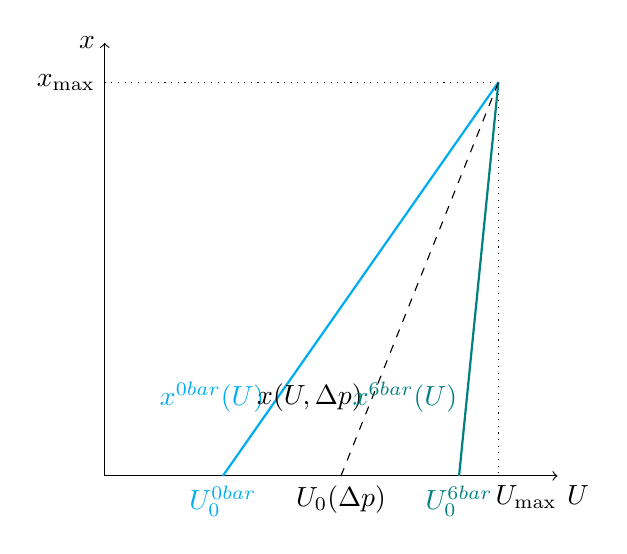
\begin{tikzpicture}[scale=.5]
    % Define the nodes
    \draw [<->] (11.5,0) node[below right] {$U$} -- (0,0) -- (0,11) node[left] {$x$} ; % Coordinates
     %Draw the lines
    \draw [dotted] (0,10) node[left] {$x_{\max}$} -- (10,10) -- (10,0) node [below] {$\qquad U_{\max}$}; % Rechts oben Hilfslinien
    \draw [thick, cyan]  (3,0) node[below]{$U_0^{0\unit{bar}}$} -- (10,10); % 0Bar Linie
    \draw [thick, teal]  (9,0) node[below]{$U_0^{6\unit{bar}}$} -- (10,10); % 6Bar Linie
    \draw [dashed] (6,0) node[below]{$U_0(\Delta p)$} -- (10,10); % 3bar Linie
    \node [cyan, left] at (4.3,2) {$x^{0\unit{bar}}(U)$};
    \node [left] at (6.8,2) {$x(U,\Delta p)$};
    \node [teal, left] at (9.2,2) {$x^{6\unit{bar}}(U)$};    
   \end{tikzpicture}
%   \caption{Illustration of the linear approximation of the measured curves}
%   \label{fig:linapprox}
% \end{figure}

  
 \end{frame}


 
%%% Local Variables:
%%% mode: latex
%%% TeX-master: "SMC4Students"
%%% End:
